% Phần mở đầu chương
% Phần mở đầu chương
Chương này trình bày quá trình thiết kế và triển khai giải pháp định tuyến dựa trên thuật toán Gradient cho giao thức BLE Mesh trên vi điều khiển nRF54L15. Giải pháp được triển khai thông qua việc phát triển một Vendor Model có tên Gradient Server Model có chức năng định tuyến dữ liệu, hoạt động song song với các SIG Model chuẩn của BLE Mesh.

\section{Kiến trúc tổng thể}
\label{sec:architecture}

\subsection{Tổng quan Gradient Server Model}

Gradient Server Model là một Vendor Model được thiết kế để triển khai thuật toán định tuyến Gradient trên nền tảng BLE Mesh. Model này hoạt động song song với các model chuẩn của BLE Mesh, tận dụng cơ chế truyền tin của BLE Mesh đồng thời bổ sung thêm logic định tuyến thông minh dựa trên giá trị gradient.

\begin{figure}[h!]
    \centering
    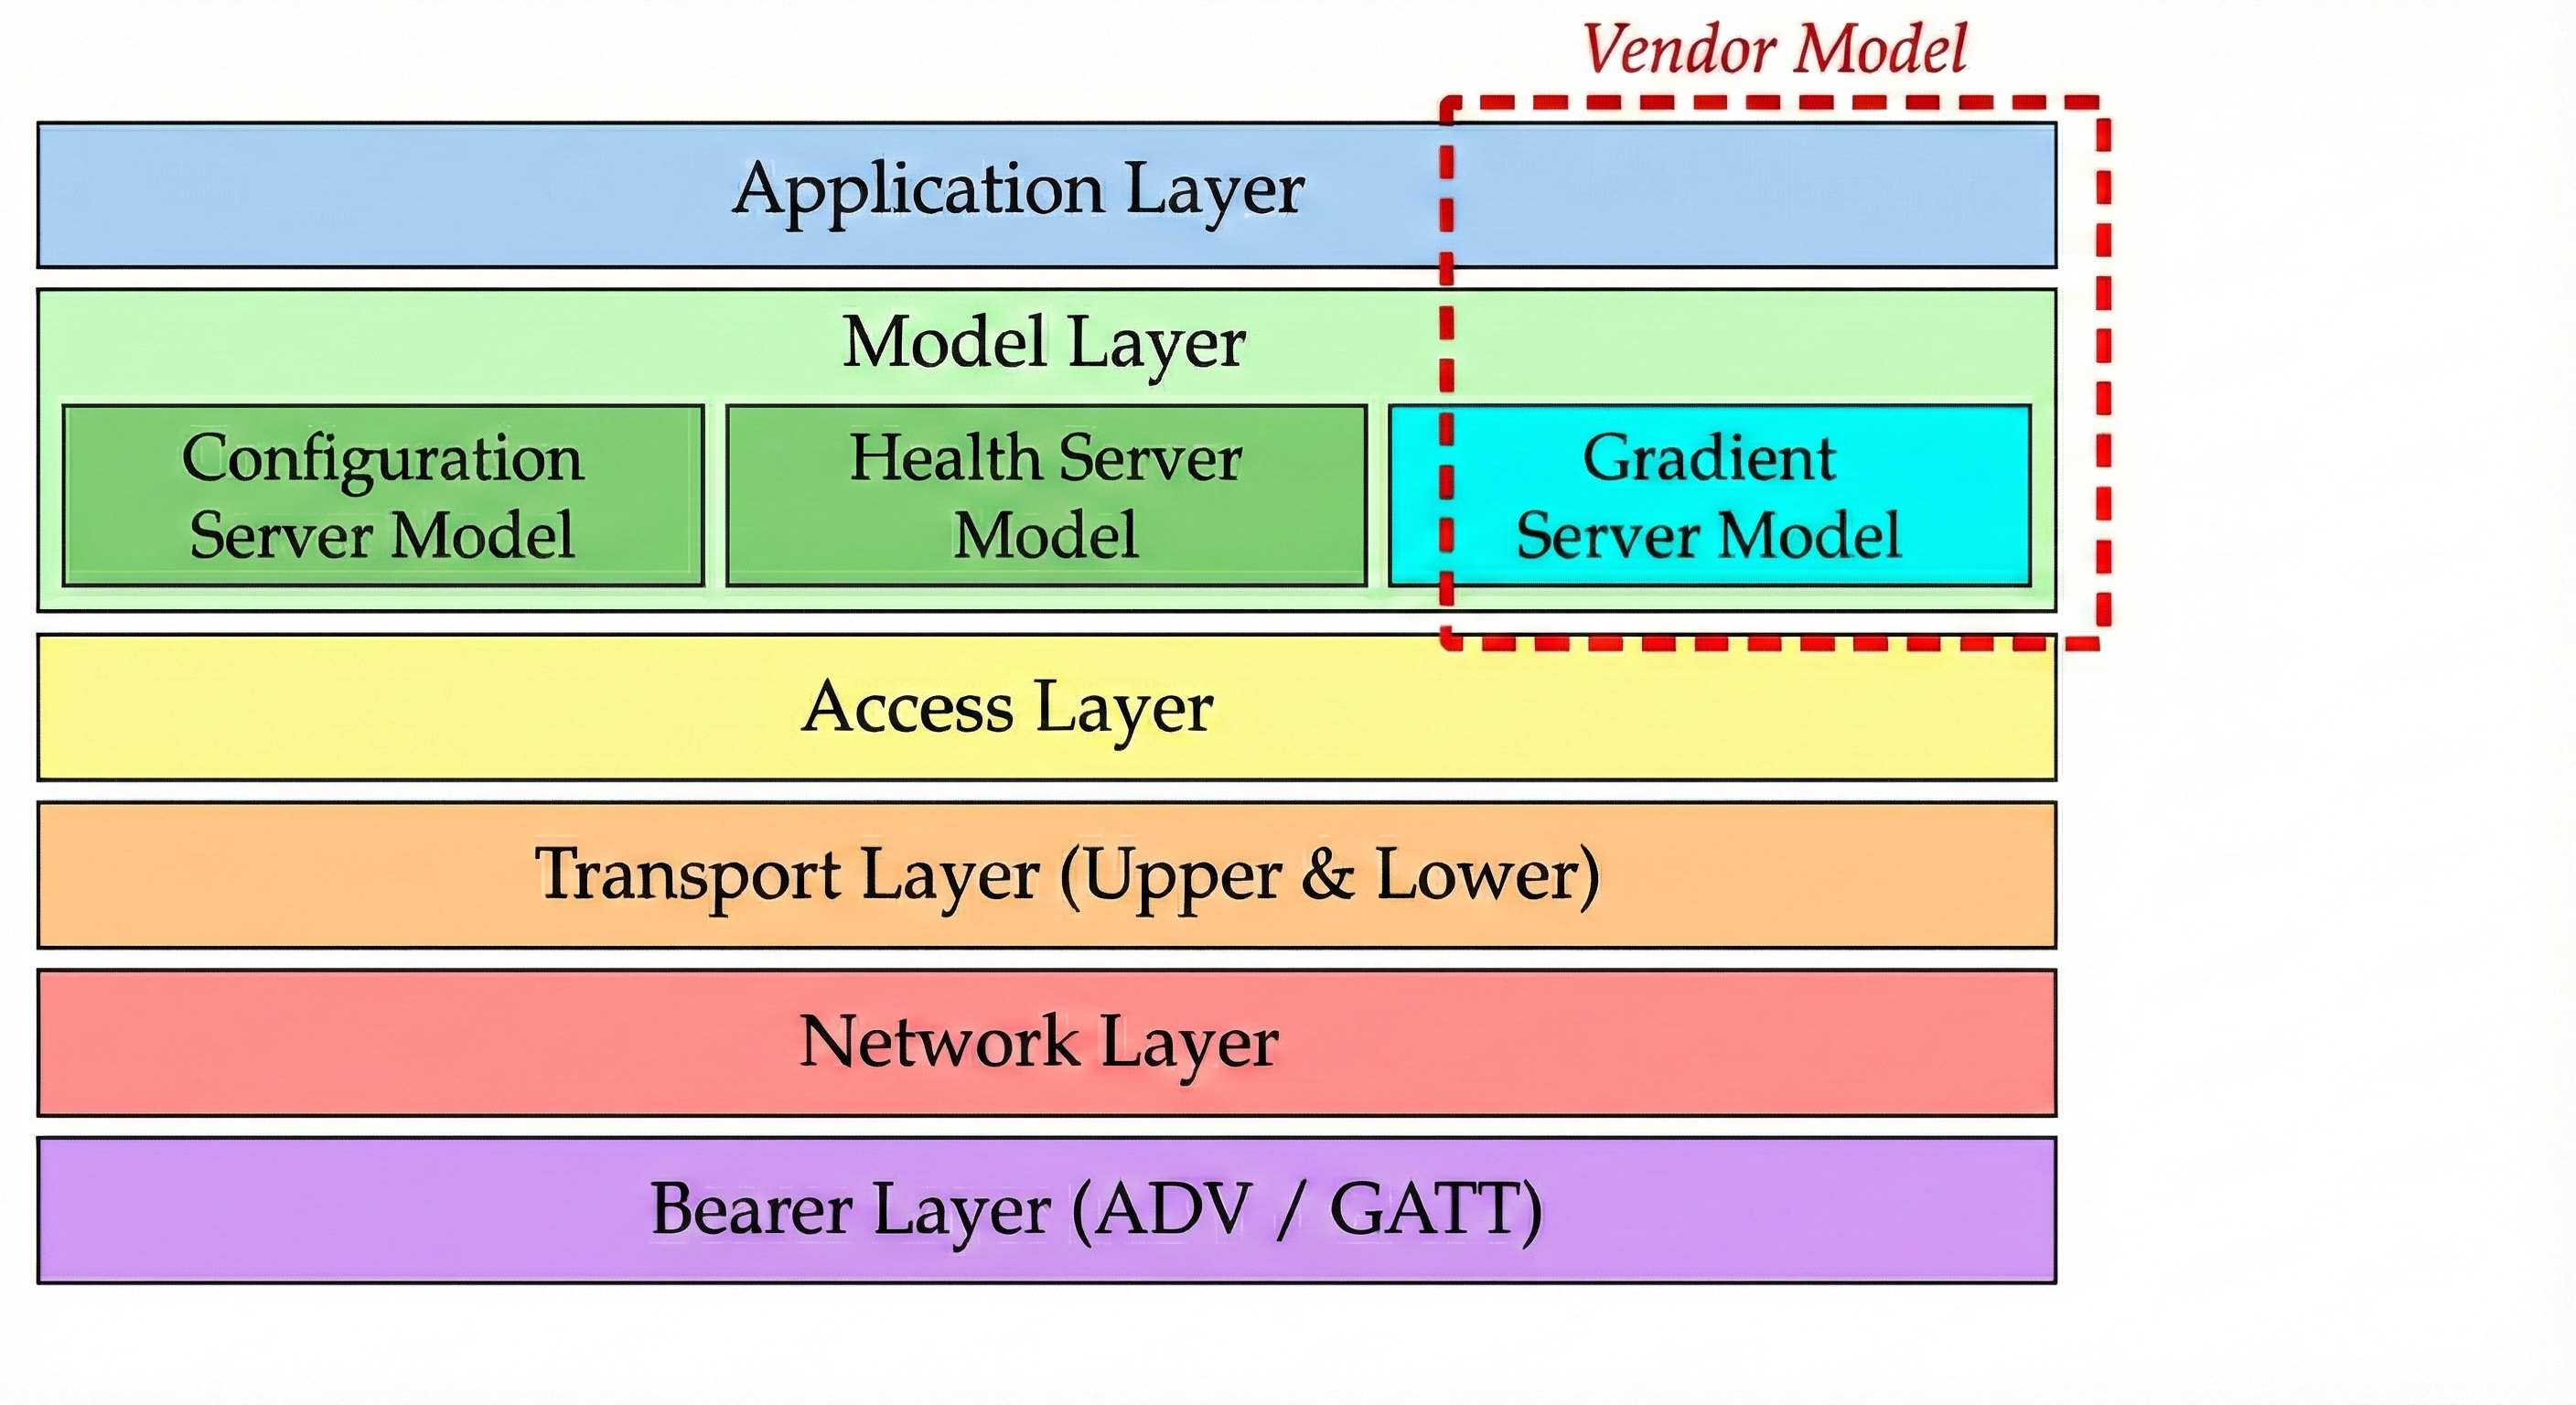
\includegraphics[width=0.75\textwidth]{chapter3/image/Gradient_model.png}
    \caption{Vị trí của Gradient Server Model trong kiến trúc BLE Mesh}
    \label{fig:gradient_model_stack}
\end{figure}

Hình \ref{fig:gradient_model_stack} minh họa vị trí của Gradient Server Model trong kiến trúc BLE Mesh. Model này được triển khai tại Model Layer, hoạt động song song với các SIG Model chuẩn như Configuration Server và Health Server. Là một Vendor Model, Gradient Server Model sử dụng Company ID của Nordic Semiconductor và có thể định nghĩa các opcode và message format riêng.

\subsection{Cấu trúc Gradient Server Model}

Gradient Server Model được thiết kế theo kiến trúc module hóa, bao gồm các thành phần chính: States (trạng thái), Message Handlers (hàm xử lý gói tin), và các cấu trúc dữ liệu hỗ trợ. Mỗi thành phần đảm nhiệm một chức năng cụ thể trong quá trình định tuyến và chuyển tiếp dữ liệu.

\begin{figure}[h!]
    \centering
    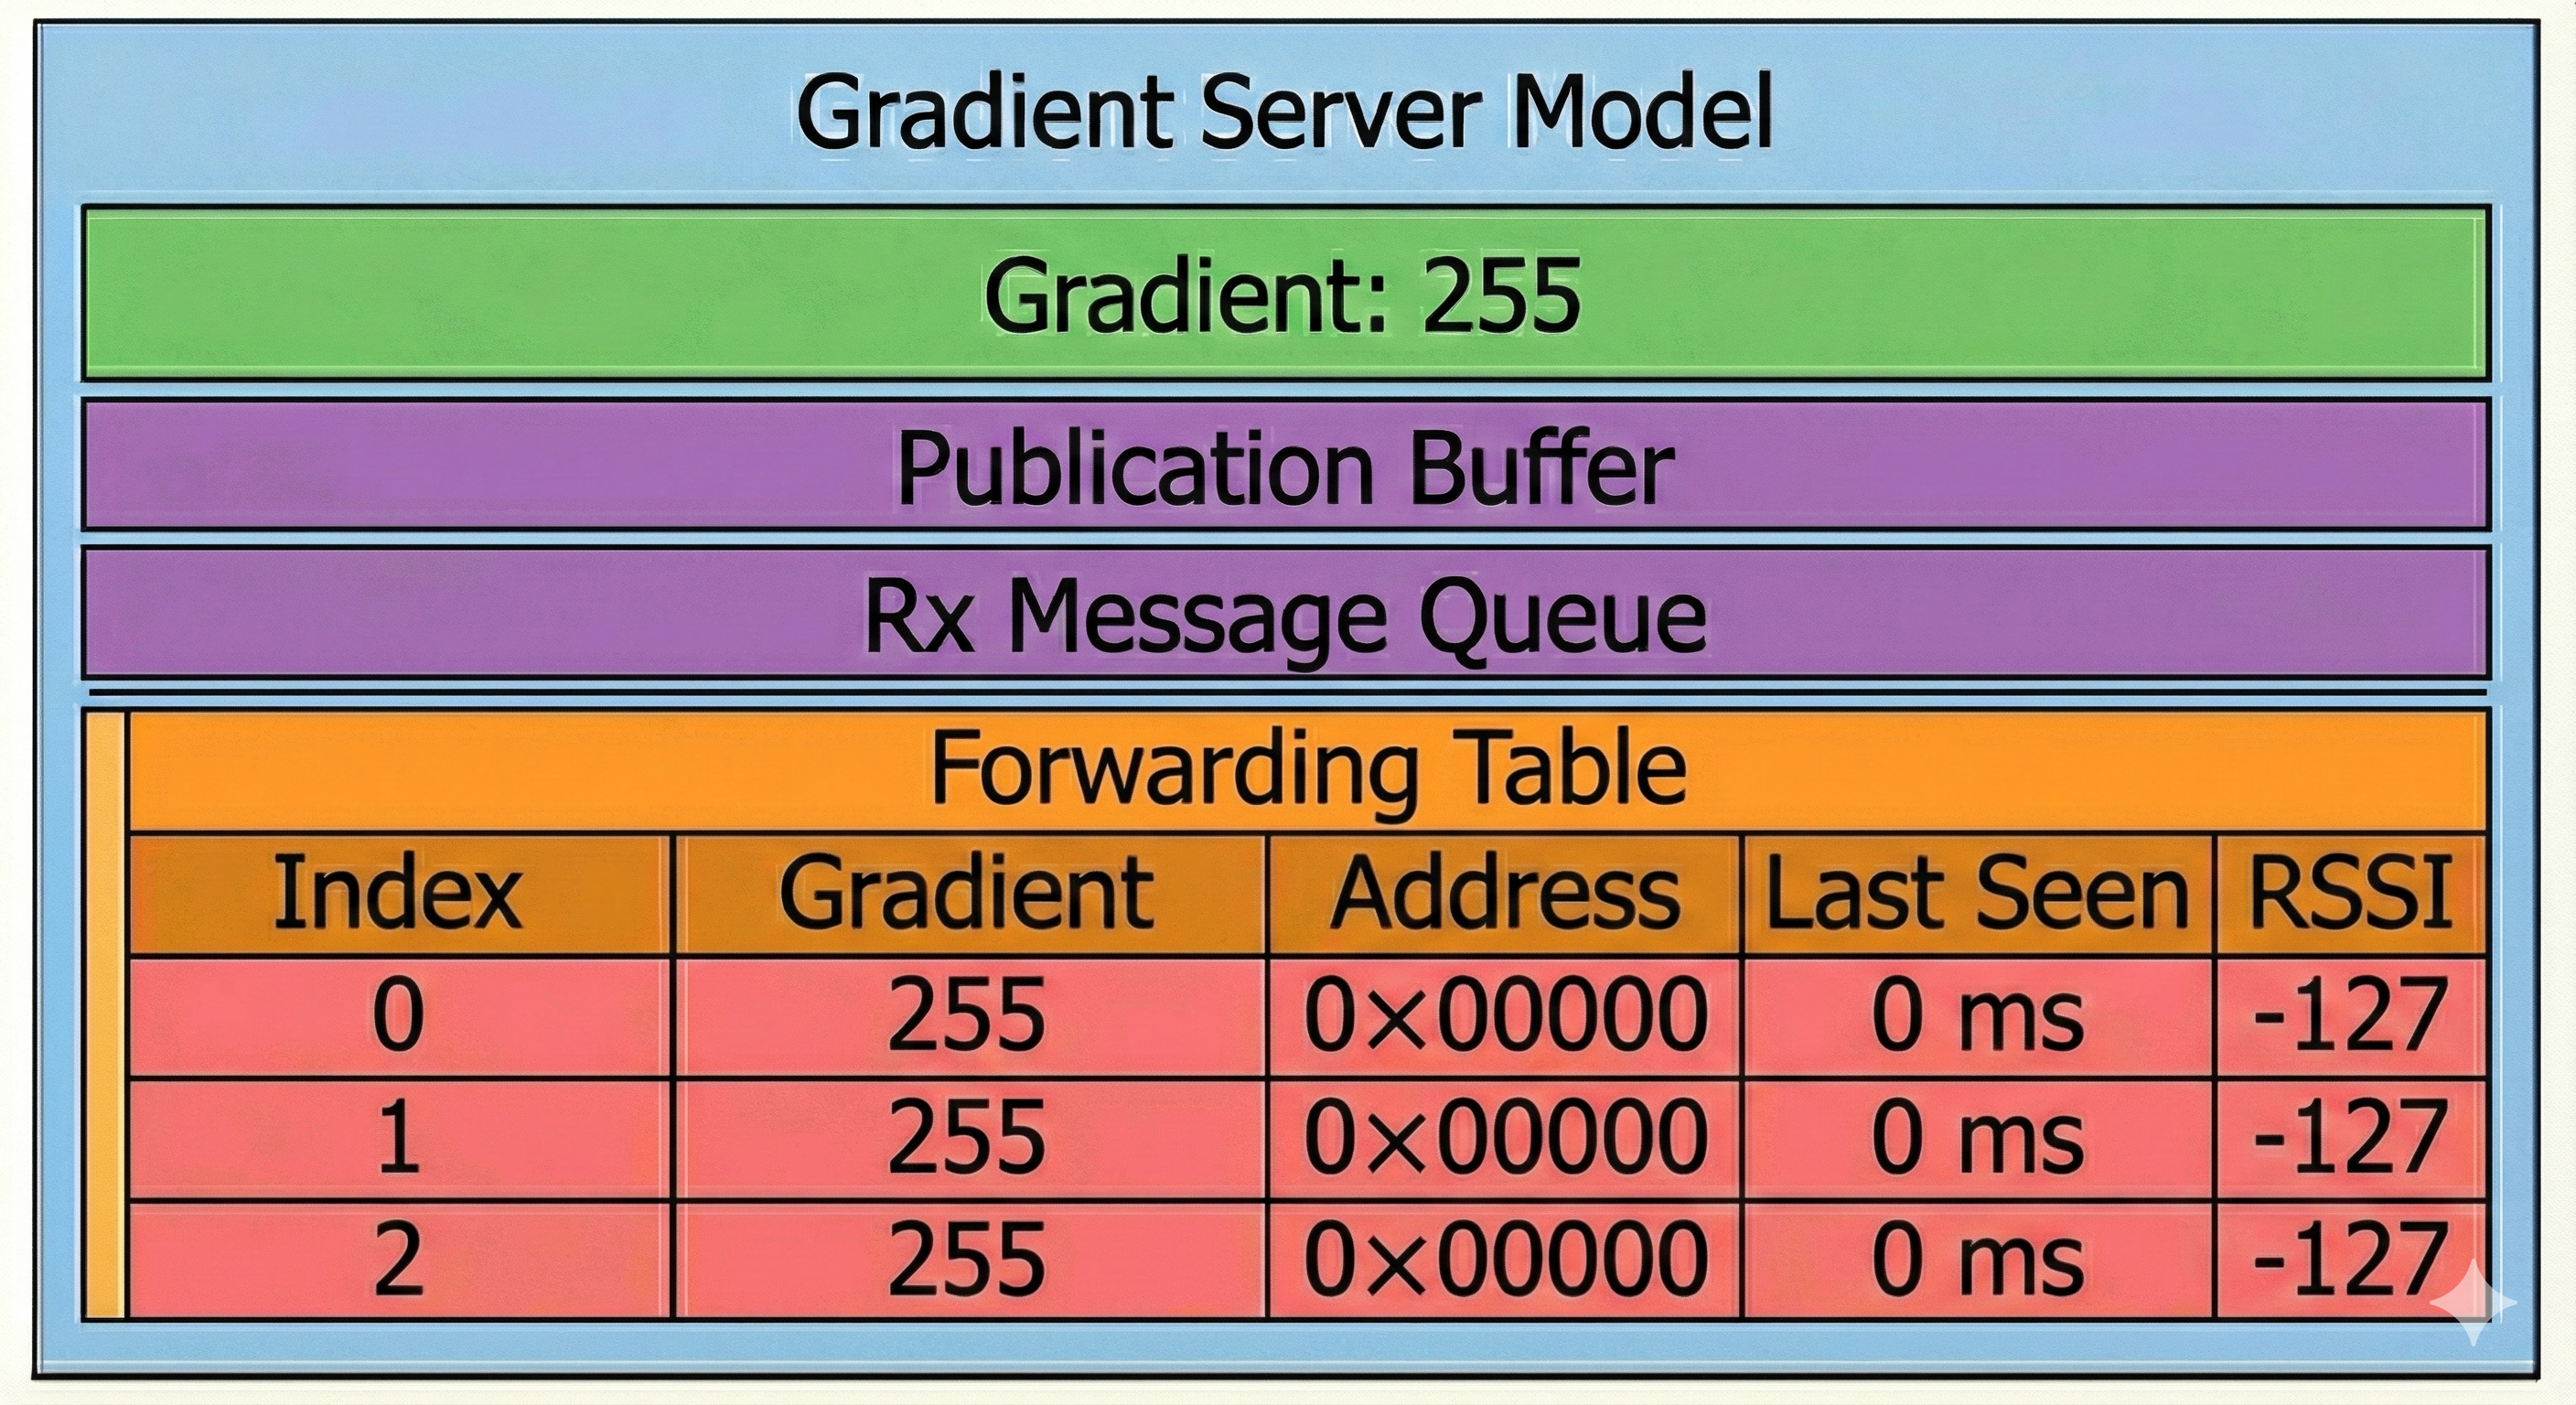
\includegraphics[width=0.9\textwidth]{chapter3/image/Gradient_model_structure.png}
    \caption{Cấu trúc nội bộ của Gradient Server Model}
    \label{fig:gradient_model_structure}
\end{figure}

\subsubsection{States (Trạng thái)}

States là các biến trạng thái được lưu trữ trong mỗi node, phản ánh tình trạng hiện tại của node trong mạng và cung cấp thông tin cần thiết cho việc ra quyết định định tuyến.

\textbf{Gradient:} Đây là giá trị số nguyên 8-bit (uint8\_t) biểu thị khoảng cách logic từ node hiện tại đến sink node. Sink node - điểm thu thập dữ liệu trung tâm của mạng - luôn có gradient bằng 0. Khi một node mới tham gia mạng hoặc khởi động lần đầu, giá trị gradient được khởi tạo bằng 255, biểu thị rằng node chưa có đường đi hợp lệ đến sink. Giá trị này sẽ được cập nhật khi node nhận được thông tin gradient từ các node lân cận. Gradient đóng vai trò then chốt trong thuật toán định tuyến: dữ liệu luôn được chuyển tiếp theo hướng gradient giảm dần, đảm bảo cuối cùng sẽ đến được sink node.

\textbf{Forwarding Table:} Đây là cấu trúc dữ liệu quan trọng nhất của Gradient Server Model, lưu trữ thông tin về tất cả các node lân cận có gradient lớn hơn hoặc bằng node hiện tại mà node hiện tại có thể giao tiếp trực tiếp. Mỗi entry trong bảng chứa các trường thông tin sau:

\begin{itemize}
    \item \textit{Address (2 bytes):} Địa chỉ unicast của node lân cận theo chuẩn BLE Mesh. Địa chỉ này được sử dụng để xác định đích đến khi chuyển tiếp gói tin.
    
    \item \textit{Gradient (1 byte):} Giá trị gradient của node lân cận. Thông tin này được cập nhật mỗi khi nhận được gói tin GRADIENT\_STATUS từ node đó. Gradient của neighbor là tiêu chí chính để chọn next-hop trong quá trình định tuyến.
    
    \item \textit{RSSI (1 byte):} Chỉ số cường độ tín hiệu nhận được (Received Signal Strength Indicator), đo bằng dBm. RSSI phản ánh chất lượng liên kết vật lý giữa hai node. Giá trị RSSI cao hơn cho thấy liên kết tốt hơn. Thông tin này có thể được sử dụng như tiêu chí phụ khi có nhiều neighbor có cùng gradient value.
    
    \item \textit{Last Seen Timestamp (4 bytes):} Thời điểm gần nhất nhận được gói tin từ node lân cận, đơn vị ms và mốc thời gian tham chiếu kể từ khi hệ thống khởi động. Timestamp này được sử dụng để phát hiện các node đã rời khỏi mạng hoặc mất kết nối. Nếu một neighbor không gửi bất kỳ gói tin nào trong một khoảng thời gian timeout, entry tương ứng sẽ bị xóa khỏi bảng.
\end{itemize}

Forwarding Table được cấu hình với kích thước tối đa cố định là 3 entry để đảm bảo sử dụng bộ nhớ hiệu quả trên các vi điều khiển có tài nguyên hạn chế. Số lượng entry trong bảng có thể được thiết lập tùy vào cấu trúc mạng cụ thể khi triển khai. Khi bảng đầy, thuật toán sẽ so sánh gradient và RSSI của các entry để quyết định thay thế hoặc không.

\subsubsection{Message Handlers (Hàm xử lý gói tin)}

Message Handlers là các hàm callback được gọi khi Gradient Server Model nhận được gói tin từ BLE Mesh stack. Mỗi loại gói tin có một handler tương ứng để xử lý logic cụ thể.

\textbf{Hàm xử lý gói tin GRADIENT\_STATUS:} Đây là handler quan trọng nhất, chịu trách nhiệm cập nhật thông tin gradient trong mạng. 

\textbf{Hàm xử lý gói tin DATA:} Handler này chịu trách nhiệm nhận và chuyển tiếp các gói tin dữ liệu thu thập từ cảm biến. 